
\item A point source $S$ is placed at the bottom of a transparent block of height $10\ mm$ and refractive index $2.72$. It is immersed in a lower refractive index liquid as shown in the figure. It is found that the light emerging from the block to the liquid forms a circular bright spot of diameter $11.54\ mm$ on the top of the block. The refractive index of the liquid is
    \begin{center}
        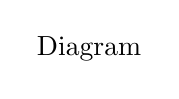
\begin{tikzpicture}
            \node at (0, 0) {Diagram};
            % Note: The actual diagram should replace this placeholder
        \end{tikzpicture}
    \end{center}
    \begin{tasks}(2)
        \task \(1.21\)
        \task \(1.30\)
        \task \(1.36\)
        \task \(1.42\)
    \end{tasks}
